%!TEX root = ../main.tex

% Judgement and analysis in planning: Mature analysis and judgement in planning showing flexibility and high awareness of contingencies, efficiency and monitoring. Fully comprehensive risk analysis and contingency planning

% Analysis of the problem: Full consideration has been given to analysis alternatives and an entirely appropriate and effective analysis of the problem results. Depth in judgement and final choices, and effective reativity in analysis

% Selection and justification of processes, methods and tools: Real depth of insight is shown, with discerning judgement in final choices, demonstrating unusual insight and very effective, creative approach to the project. Methods/technology are totally appropriate to the objectives, with a thorough, considered justification for their selection, and are used with flair.

% Appropriateness of solution design: Full consideration has been given to design alternatives and an entirely appropriate and effective solution results. Real depth of insight is shown, with discerning judgement in final choices, demonstrating unusual insight and very effective creativity in designing a solution to the problem that is as close to an optimum solution as can be expected.

% Appropriateness of evaluation design: Full consideration has been given to evaluation alternatives and an entirely appropriate and effective evaluation approach results. Real depth of insight is shown into the factors affecting the quality of the solution, with discerning judgement in final choices, demonstrating unusual insight and very effective creativity in designing effective evaluation at all stages of development.
\chapter{Methodology}
\label{chap:methodology}

To ensure transparency and reproducibility of the outcomes, this chapter articulates the methodology used in the organizational, structural and procedural aspects of the dissertation. Firstly, it introduces the process of initial analysis and planning that sets the base for the present work. After this, it describes the methodology used in carrying out the research and literature review. The following subsection shows insight into the process of translating objectives into requirements and the design decisions taken. The penultimate subsection will discuss the technical details of the artifact. It will increase the resolution at which the design has been presented. Finally, the last subsection will expand over the methodology of evaluation used throughout this dissertation.

\section{Planning and initial analysis}
A compulsory prerequisite of the planning and initial analysis phase is problem definition. The low-resolution problem definition developed at this stage serves as the cornerstone for further design and analysis. After the problem definition is produced, research is carried out to confirm its existence and particularities. This is done to reduce the discrepancy between the subjective view on the problem and its objective state defined by the literature.

From research on the problem of phishing and how it's impact maps on different areas, a formal compilation of objectives has been extracted as shown in Table \ref{tab:OBJECTIVES}. The next stage is designing a bare but viable solution specification around the aforementioned objectives. Based on this specification, the necessary research and procedures identified and mapped over a Gantt chart with an educated time estimate attributed to each. The final step of the initial analysis and planning is to perform a risk analysis. This reduces the probability of confronting an obstacle that has not been identified, thus having no planned mitigation.

To better visualize the planning and initial analysis phase, an illustration of the sequence of procedures is presented in Figure \ref{fig:INITIAL_ANALYSIS}.

\begin{figure}
	\centering
	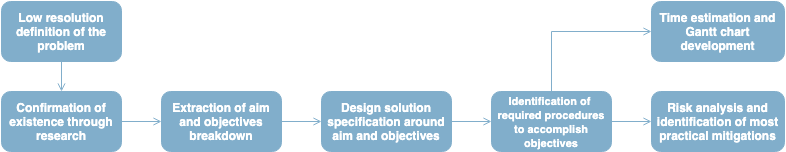
\includegraphics[width=1\textwidth]{initial_analysis.png}
	\caption{Illustration of initial analysis}
	\label{fig:INITIAL_ANALYSIS}
\end{figure}

\section{Research methodology}
The target of the research and literature review shifted from one chapter to another. However, the aim has constantly been to develop an in-depth and high-resolution image of the subject matter and base the work presented upon previous studies rather than suppositions. Throughout this dissertation, the systematic process used in doing the literature review is comprised of two procedures.

The first procedure dictates that the research should begin by firstly identifying a reputable and well established study. This paper is thoroughly read and the information relevant is extracted and processed accordingly.
The second procedure is used to deepen the understating of the subject. Based on the paper identified by procedure one, the points of interest are followed by spidering through the references. When the process of spidering brings in focus papers that are not relevant to the aim, the research should return to procedure one.

Following this method ensures that by the end of the research phase, there will be a clear and in-depth understanding of the status quo in the subject of interest. In addition, the papers included in the background study have received a greater level of attention to produce a pertinent appraisal of the work they present.

% DESING-OLD: The second step is the identification of highly performant machine learning-based solutions and the study of their design. Most of the research on anti-phishing detection systems presents comparisons of the inner workings of the proposed solution with other related implementations. Based on these, the set of the most effective mechanisms identified can be implemented to work together towards classifying URLs. Besides this, the experimentation phase includes the training of different machine learning models, calibrating parameters, changing training data, and the comparison of results. 
% It's design is built and refined through a loop of research and experimentation

\section{Artefact design and development}
The functional outcome of this dissertation is composed of two artifacts. The first is the Google Safe Browsing evaluation tool used to uncover Safe Browsing's classification accuracy. The second artifact is the classifier used to predict whether an URL points to a phishing page or not.

\subsection{Evaluation tool}
The evaluation tool is written in Python and uses the Selenium framework for browser automation. Python is used due to it's extensive support and ease of use. The selenium framework is chosen because of it's reputation in browser automation testing and expansive documentation. The target of the evaluation tool is to mimic a user clicking on a phishing link. This is done in order to capture effectiveness in a real-world scenario. The alternative to this is using Google's Safe Browsing API for checking.

The URLs used in the evaluation process are the latest provided by Phishtank at the moment of evaluation. These are confirmed to be online and malicious by the PhishTank community. The test executed for each of the malicious URLs starts with loading the default profile of the Google Chrome user. Experimentation with the browser has shown that not loading a user's profile delivers unreliable results. After doing so the URL is opened and the page shown by the browser is studied. When a page is classified as malicious, the browser displays a custom page with a warning as shown in Figure \ref{fig:PHISHING_PREVENTED}. To verify whether the browser correctly classifies the URL, the tool searches the page's source code for Google's license details present in the warning page. If the browser shows the warning page overlay, the classification is marked as a true-positive, otherwise it is recorded as a false-negative.

\begin{figure}
	\centering
	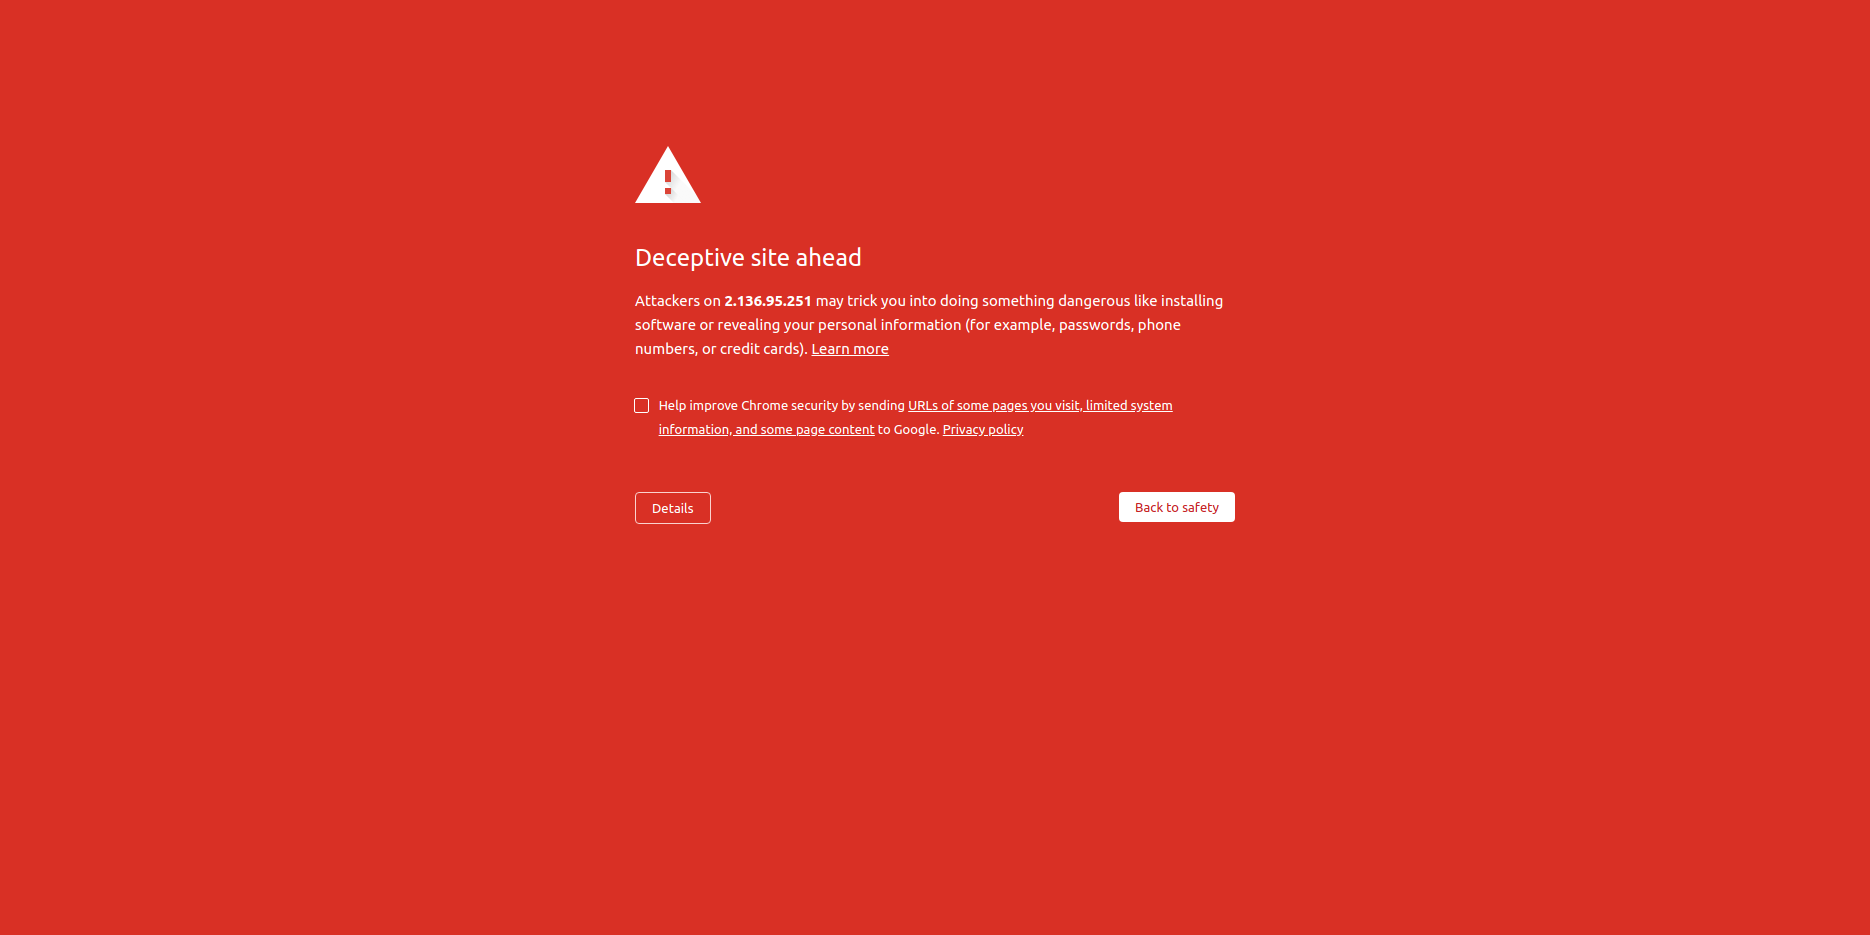
\includegraphics[width=1\textwidth]{malicious.png}
	\caption{Example of browser's warning page overlay}
	\label{fig:PHISHING_PREVENTED}
\end{figure}

\subsection{The classifier}
The classifier is the main artefact, set to accomplish the dissertation's aim of delivering better protection against phishing than the most popular browsers do. The selected approach in designing a competitive anti-phishing detection system is through the identification of key performance indicators that are efficient in phishing URL classification. Naturally, the first step in designing the artifact is corroborating information from a wide range of studies on the indices that achieve high classifications accuracy. Following this, the algorithms are compared and the best performing one is selected
Given the multi-layered structure of the artifact, each layer has it's own implementation specification and is discussed separately.

The machine learning models compared in this dissertation are trained using Python and SciKitLearn library. Python is chosen over other programming languages as it is considered the de-facto in the field of data science. The SciKit library is used as an abstraction of the actual machine learning algorithms. By alleviating the complexity of the implementation of machine learning algorithms used, the saved time is allocated towards experimentation and calibration.

The wrapper and the set of additions are implemented in using the same programming languange. Although better performance can be achieved using a different languange, this is done to preserve continuity throughout the artefact.

TO BE REVISITED
%The development lifecycle

\section{Evaluation methodology}
The evaluation of browser's anti-phishing detection mechanism is done in two phases. Firstly the browser will be assessed using newly discovered phishing URLs. After a week of the aforementioned evaluation, the browser will be assessed again using same data. The rationale behind this lies in the study of how browsers evolve their defenses regarding old phishing data.

The evaluation of the machine learning models is based on a set of metrics that cover all the performance areas. In addition to covering performance areas, the proposed set makes the process of identifying flaws in callibration easier. Besides these, the evaluation methodology will coincide with the one presented by some of the studies discussed in the backgroud study. This is done with the aim of achieving consistency and offering a fair comparison with existent work.\newline


\begin{equation}
	\label{eq:PRECISION}
	Precision = \frac{TP}{TP+FP}
\end{equation}
\begin{equation}
	\label{eq:SENSITIVITY}
	Sensitivity = \frac{TP}{TP+FN}
\end{equation}
\begin{equation}
	\label{eq:FMEASURE}
	F-Measure = 2*\frac{Precision * Sensitivity}{Precision + Sensitivity}
\end{equation}
\begin{equation}
	\label{eq:ACCURACY}
	Accuracy = \frac{TP+TN}{TP+TN+FN+FP}
\end{equation}
\newline

The metrics presented in \ref{eq:PRECISION},\ref{eq:SENSITIVITY},\ref{eq:FMEASURE} and \ref{eq:ACCURACY} represent key statistical concepts. A system is said to be precise (\ref{eq:PRECISION}) when it delivers a high level of correct prediction values. . Sensitivity \ref{eq:SENSITIVITY}, also known as recall, outlines system's predisposition in classifying an legitimate URL as being malicious. As the system grows in sensitivity, it reduces the number of false-negatives it produces. To put things in perspective, precision is the ratio between all adequate classification errors and all classification errors, whereas recall is the ratio of all classification errors and all existing errors.
The F-Measure (\ref{eq:FMEASURE}) is the harmonic mean of precision (the number of correct predictions) and robustness (works well with URLs difficult to classify). It is a composed metric which penalizes the extreme values and is meant to provide a single measurement for a system which illustrates the level of optimization. Finally, the accuracy (\ref{eq:ACCURACY}) measures the ratio of true-positives and true-negatives.

The final evaluation of the produced classifier is done in comparison to the evaluation tool's results. It is based on the same data set and same metrics to eliminate any variables that may appear between evaluation methods.

% =========================================================================================================
% Skipped compiling instructions
\iffalse
1st module Whitelist/Blacklist
		Hash urls and do lookups as cheap as possible
2nd module Heuristics
		Compile a set of heuristics from the papers based on performance
3rd module Visual similarity/Content evaluation
		Think about studying the visual similarity or some content evaluation if feasible
4th module Machine learning
		use Cohen's kappa static to measure agreement between stacked machine learning algos
		URL classifier (supervised learning)
		Domain classifier (trained with https://github.com/elceef/dnstwist)
		DGA classifier (optional)

Figures must be correctly numbered with captions and paragraph text should not be wrapped around figures - same rules apply to tables. An example of figures can be found below.
\begin{figure}[t]
	\centering
	
\includegraphics[width=0.45\textwidth]{unilogo.jpg}
	\caption{Bournemouth University}
	\label{fig:BULogo3}
\end{figure}
You should always start with an overview (Heading 2 style) to tell what this chapter is about and finkish with a summary (Heading 2 style) to tell what has been covered in this chapter.

This chapter is about discussing your project planning and methodology. Note that your chosen methodology should be based on the constraints and complexity of your project instead of some common senses with no link to your own project.]
\fi